% Airborne ice-penetrating radar data has been used to explore past ice sheet evolution and flow as well as to indirectly probe modern ice sheet boundary conditions. In order to do so, it is useful to determine the age of radar-observed englacial layers to provide constraints on the timing of features indicative of past change within the ice. More than a dozen surveys over the last several decades have provided extensive coverage of central West Antarctica, including the Thwaites Glacier catchment and Marie Byrd Land regions. These surveys pass near the Byrd (80.0167$^\circ$S, 119.5167$^\circ$W) and WAIS Divide (79.48$^{\circ}$S, 112.11$^{\circ}$W) ice cores, making it possible to correlate ice core chronologies with observed englacial layers at depth. 

% The WAIS Divide ice core has been dated to 68 ka and the Byrd ice core has been dated to 91 ka, thus providing the potential for dating West Antarctic englacial ice through most of the Last Interglacial cycle. However, while a robust age-depth chronology is available for the recently-drilled WAIS Divide ice core, the Byrd ice core chronology -- the first deep core to be drilled in Antarctica -- lacks sufficient error analysis. We derive uncertainty for the Byrd ice core chronology using a combination of ice flow modeling and correlation of layers traced between the well-dated WAIS Divide ice core and the Byrd ice core. Additionally, the contribution of uncertainty in layer depth observed from ice-penetrating radar has not been computed for the West Antarctic. Using specifications of the radar system, we quantify radar depth uncertainty and include it when assigning ages to radar-observed layers of interest.

% Age registration of englacial layers is most practical for layers which can be tracked continually both to an ice core and throughout a large domain. We identify 9 such layers at the WAIS Divide ice core and 10 layers at the Byrd ice core which are dated and tracked for hundreds of line-km in central West Antarctica. The result is isochronous surfaces which reveal evidence of deformation in the ice sheet and could identify areas of changes in accumulation, flow, or subglacial boundary conditions. This three-dimensional view of the inside of the West Antarctic ice sheet provides a new avenue to validate ice sheet models and explore past behavior and dynamics of the ice sheet. 

% \begin{figure}[!h]
% %\begin{center}
% \centering
% 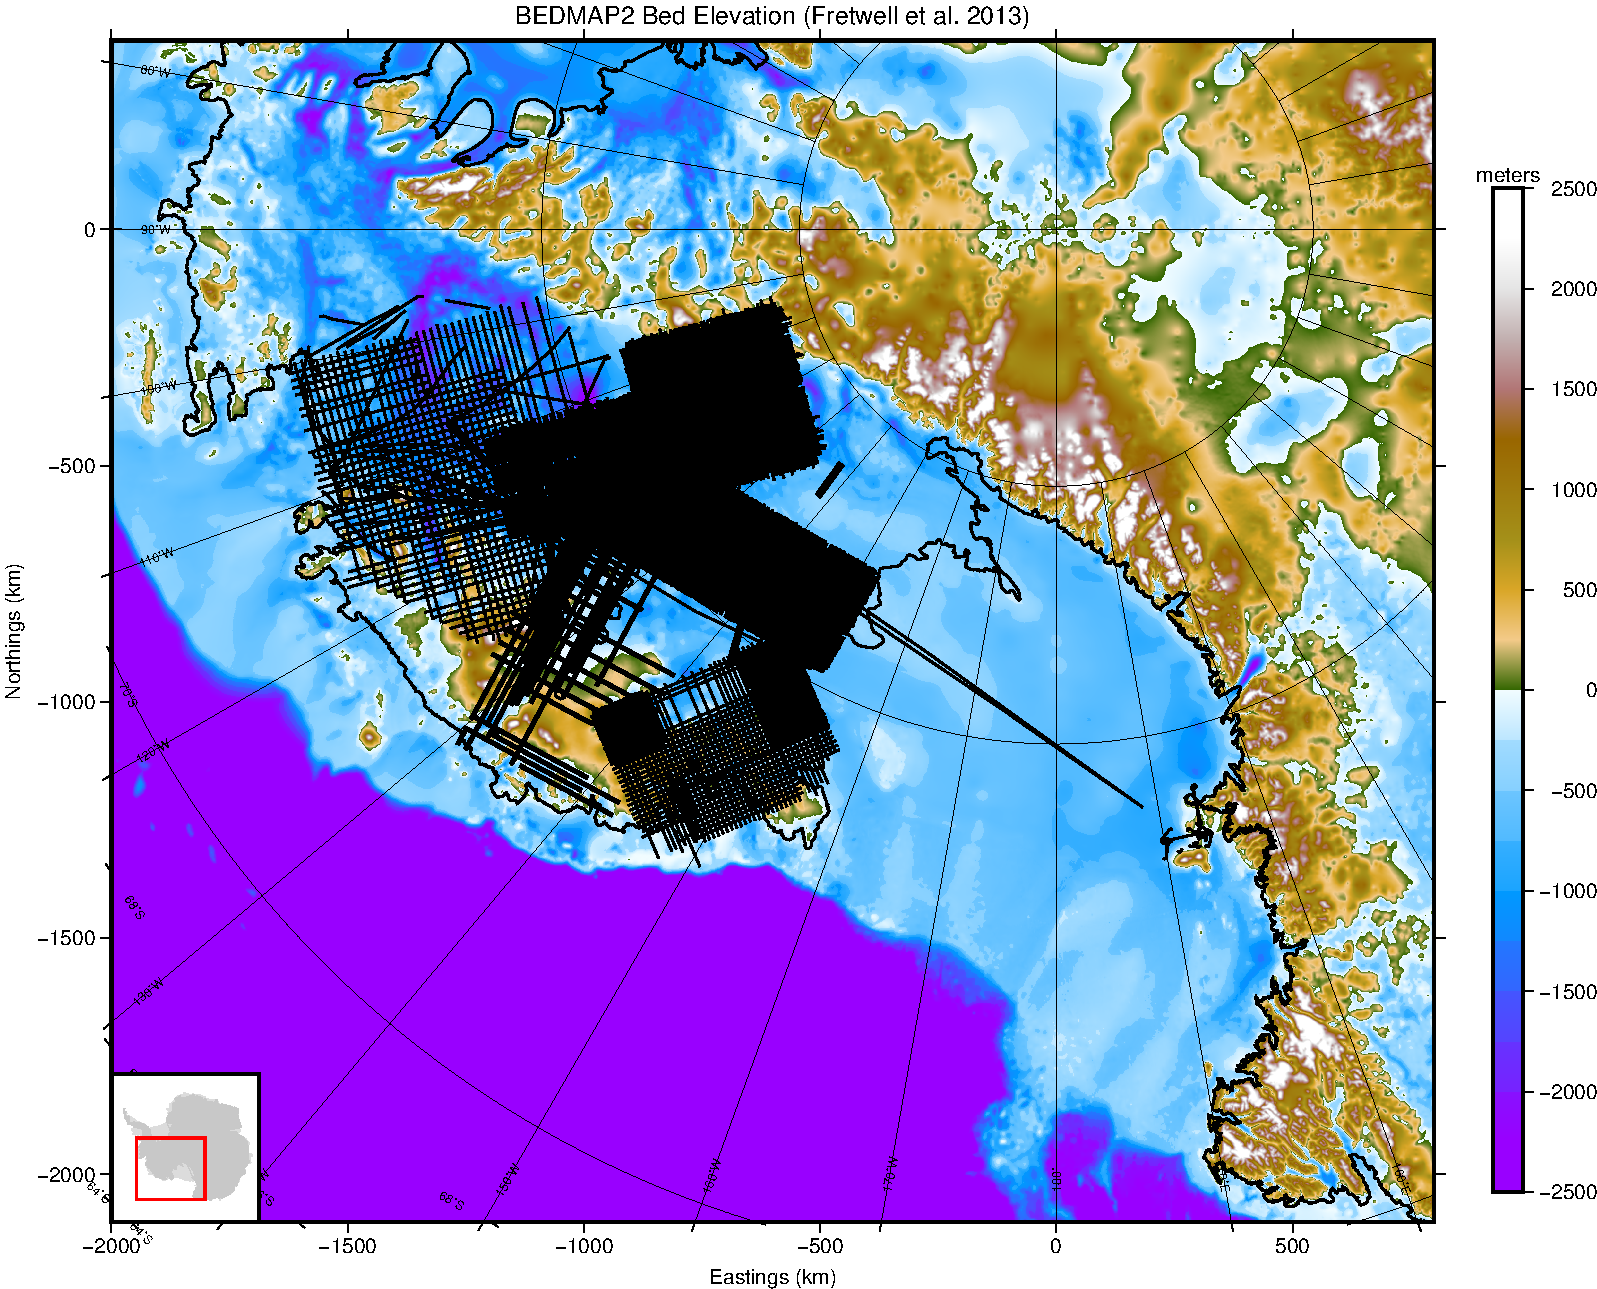
\includegraphics[scale=0.3]{figures/Fig1_WAISall_bed2}
% %\captionsetup{width=.9\textwidth}
% \caption[]{Map of central West Antarctic with available airborne geophysical radar surveys (black lines) and (\textbf{will be updated to have:} WAIS Divide and Byrd ice core locations (blue triangles) overlain. Gray shading is surface elevation according to Fretwell et al. 2013. }
% %\end{center}
% \label{fig:radarmap}
% \end{figure}


The Byrd ice core (80.0167$^\circ$S, 119.5167$^\circ$W) was the first to be drilled to bedrock in Antarctica \citep{gow1968}. The proximity of the core to fast-changing ice of both the Siple and Amundsen Sea coasts in West Antarctica make it a potentially important source of information in studies of the response of the West Antarctic Ice Sheet (WAIS) to changing climatic conditions. Extensive radar surveys passing near the core site make it particularly useful for dating paleo ice dynamics observed in the central WAIS. Dated englacial radar data enables information from the entire ice volume--rather than only surface observations--to constrain ice dynamics in the central WAIS, including the Thwaites Glacier catchment and Marie Byrd Land.

While the Byrd ice core has been dated to more than 90ka \citep{}, nearly back to the Last Interglacial, the chronology lacks estimates of uncertainty in age and depth. Here we use a Bayesian technique to compute a probabilistic chronology for the Byrd ice core which is constrained by existing ice core chronology results. This method inverts for probability distributions of ice sheet parameter values consistent with the recorded ice core chronology. 

We use the modeled chronology to assign ages to englacial reflectors traced through the central WAIS. These reflectors encode information about ice sheet boundary conditions and paleo ice dynamics \citep[e.g.][]{}. They are the result of dielectric contrasts in the ice due to variations in composition, crystal fabric, temperature, and other ice properties. Each continuous reflector is assumed to be the result of a distinct surface deposition episode with a distinguishable dielectric signature and is therefore assumed to be isochronous \citep{fujita2000}. 

The isochronous nature of englacial reflectors implies that assigning an age to each reflector at the Byrd ice core site effectively dates the reflector anywhere it can be continuously traced in the region. This allows for extensive age registration throughout the ice column and radar survey domain and also for validation of our results at the Byrd ice core with the recently-drilled WAIS Divide ice core chronology, as has been done in East Antarctica \citep{cavitte2016}. The WAIS Divide ice core (79.48$^{\circ}$S, 112.11$^{\circ}$W) provides an ice chronology with uncertainty quantification as far as back as 67ka \citep[][C. Buizert, personal communication]{buizert2015} and is therefore an independent validation of our improved Byrd ice core chronology. 

Having two ice cores from which to date englacial reflectors enables more extensive dating, particularly in areas of complicated basal topography where the radar isochrones experience increased discontinuity and cannot be tracked for long distances. This is the case near the Marie Byrd Land icecap, for example, where reflectors originating from the Byrd ice core site have been traced around areas of disruption due to high-relief bed terrain. In general, deeper reflectors are more difficult to track extensively in the WAIS due to lower amplitudes and higher levels of disruption due to basal processes. However, we interpolate three-dimensional isochronous surfaces for the extent of each of four observed reflectors which sample the ice depth. The modeled chronology is used to assign ages to these surfaces.


%The estimated Byrd ice core chronology and published WAIS Divide ice core record are used to assign dates to englacial radar reflectors observed at the ice core sites, which are assumed isochronous \citep{cite}. These isochronous reflectors have been traced extensively throughout Central West Antarctica. As such, we leverage the ice core chronologies to date observable ice stratigraphy hundreds of kilometers from existing ice core records.


Section~\ref{byrdchronology} discusses the ice flow model used and the estimation of an age uncertainty envelope for the Byrd ice core. Section~\ref{byrdwdcompare} introduces ice-penetrating radar data collected in the region and compares the age of selected reflectors determined at the Byrd and WAIS Divide ice cores. %Section~\ref{layersurfaces} explores the application of ages at the ice cores to extensive isochronous surfaces throughout West Antarctica, which can be used to analyze paleo flow and boundary conditions in the region. 
